% !TeX TS-program = pdflatex


\documentclass[a4paper]{article}

% \usepackage[default]{fontsetup}

\usepackage{fancyhdr}
\usepackage{extramarks}
\usepackage{amsmath}
\usepackage{amsthm}
\usepackage{amsfonts}
\usepackage{tikz}
\usepackage[plain]{algorithm}
\usepackage{algpseudocode}
\usepackage{enumerate}
\usepackage{tikz}

\usetikzlibrary{automata,positioning}

%
% Basic Document Settings
%  

\topmargin=-0.2in
\evensidemargin=0in
\oddsidemargin=0in
\textwidth=6.5in
\textheight=9.5in
\headsep=0.25in

\linespread{1.1}

\pagestyle{fancy}
\lhead{\hmwkAuthorName}
\chead{\hmwkClass : \hmwkTitle}
\rhead{\firstxmark}
\lfoot{\lastxmark}
\cfoot{\thepage}

\renewcommand\headrulewidth{0.4pt}
\renewcommand\footrulewidth{0.4pt}

\setlength\parindent{0pt}

%
% Create Problem Sections
%

\newcommand{\enterProblemHeader}[1]{
    \nobreak\extramarks{}{Problem \arabic{#1} continued on next page\ldots}\nobreak{}
    \nobreak\extramarks{Problem \arabic{#1} (continued)}{Problem \arabic{#1} continued on next page\ldots}\nobreak{}
}

\newcommand{\exitProblemHeader}[1]{
    \nobreak\extramarks{Problem \arabic{#1} (continued)}{Problem \arabic{#1} continued on next page\ldots}\nobreak{}
    \stepcounter{#1}
    \nobreak\extramarks{Problem \arabic{#1}}{}\nobreak{}
}

\newcommand*\circled[1]{\tikz[baseline=(char.base)]{
		\node[shape=circle,draw,inner sep=2pt] (char) {#1};}}


\setcounter{secnumdepth}{0}
\newcounter{partCounter}
\newcounter{homeworkProblemCounter}
\setcounter{homeworkProblemCounter}{1}
\nobreak\extramarks{Problem \arabic{homeworkProblemCounter}}{}\nobreak{}

%
% Homework Problem Environment
%
% This environment takes an optional argument. When given, it will adjust the
% problem counter. This is useful for when the problems given for your
% assignment aren't sequential. See the last 3 problems of this template for an
% example.
%

\newenvironment{homeworkProblem}[1][-1]{
    \ifnum#1>0
        \setcounter{homeworkProblemCounter}{#1}
    \fi
    \section{Problem \arabic{homeworkProblemCounter}}
    \setcounter{partCounter}{1}
    \enterProblemHeader{homeworkProblemCounter}
}{
    \exitProblemHeader{homeworkProblemCounter}
}

%
% Homework Details
%   - Title
%   - Class
%   - Due date
%   - Name
%   - Student ID

\newcommand{\hmwkTitle}{Homework\ \#12}
\newcommand{\hmwkClass}{Probability \& Statistics for EECS}
\newcommand{\hmwkDueDate}{2024-12-31}
\newcommand{\hmwkAuthorName}{Wenye Xiong}
\newcommand{\hmwkAuthorID}{2023533141}


%
% Title Page
%

\title{
    \vspace{2in}
    \textmd{\textbf{\hmwkClass:\\  \hmwkTitle}}\\
    \normalsize\vspace{0.1in}\small{Due\ on\ \hmwkDueDate\ at 11:59}\\
	\vspace{4in}
}

\author{
	Name: \textbf{\hmwkAuthorName} \\
	Student ID: \hmwkAuthorID}
\date{}

\renewcommand{\part}[1]{\textbf{\large Part \Alph{partCounter}}\stepcounter{partCounter}\\}

%
% Various Helper Commands
%

% Useful for algorithms
\newcommand{\alg}[1]{\textsc{\bfseries \footnotesize #1}}
% For derivatives
\newcommand{\deriv}[1]{\frac{\mathrm{d}}{\mathrm{d}x} (#1)}
% For partial derivatives
\newcommand{\pderiv}[2]{\frac{\partial}{\partial #1} (#2)}
% Integral dx
\newcommand{\dx}{\mathrm{d}x}
% Alias for the Solution section header
\newcommand{\solution}{\textbf{\large Solution}}
% Probability commands: Expectation, Variance, Covariance, Bias
\newcommand{\E}{\mathrm{E}}
\newcommand{\Var}{\mathrm{Var}}
\newcommand{\Cov}{\mathrm{Cov}}
\newcommand{\Bias}{\mathrm{Bias}}

\begin{document}


% \maketitle
% \thispagestyle{empty}
% \pagebreak

\date{
Due on Dec. 31, 2024, 11:59 UTC+8}
\title{SI 140A-02  Probability \& Statistics for EECS, Fall 2024 \\
Homework 12}
\maketitle
Read all the instructions below carefully before you start working on the assignment, and before you make a submission.
\begin{itemize}
    \item You are required to write down all the major steps towards making your conclusions; otherwise you may obtain limited points of the problem.
    \item Write your homework in English; otherwise you will get no points of this homework.
    \item Any form of plagiarism will lead to $0$ point of this homework. 
\end{itemize}
\newpage
\begin{homeworkProblem}[1]
Let $\boldsymbol{X}=\left(X_{1}, \ldots, X_{n}\right)$ be a random sample from the distribution $\mathcal{N}\left(\mu, \sigma^{2}\right)$, where both $\mu$ and $\sigma^{2}$ are unknown constants. Suppose the observed data is $\boldsymbol{x}=\left(x_{1}, \ldots, x_{n}\right)$, find both $\hat{\mu}$ (estimate of $\mu$ ) and $\hat{\sigma}^{2}$ (estimate of $\sigma^{2}$ ) through the MLE (Maximum Likelihood Estimation) rule.
\subsection{Solution}
The likelihood function is given by
$$
f(\boldsymbol{x} | \mu , \sigma^2)=\prod_{i=1}^{n} \frac{1}{\sqrt{2 \pi \sigma^{2}}} \exp \left(-\frac{\left(x_{i}-\mu\right)^{2}}{2 \sigma^{2}}\right)=\left(2 \pi \sigma^{2}\right)^{-n / 2} \exp \left(-\frac{1}{2 \sigma^{2}} \sum_{i=1}^{n}\left(x_{i}-\mu\right)^{2}\right)
$$
And we have the log-likelihood function
$$
\begin{aligned}
\ell(\mu, \sigma^{2} ; \boldsymbol{x}) &=\log L(\mu, \sigma^{2} ; \boldsymbol{x}) \\
&=-\frac{n}{2} \log \left(2 \pi \sigma^{2}\right)-\frac{1}{2 \sigma^{2}} \sum_{i=1}^{n}\left(x_{i}-\mu\right)^{2}
\end{aligned}
$$
To find the MLE of $\mu$, we take the derivative of $\ell$ with respect to $\mu$ and set it to zero:
$$
\begin{aligned}
\frac{\partial \ell}{\partial \mu} &=\frac{1}{2 \sigma^{2}} \sum_{i=1}^{n} 2\left(x_{i}-\mu\right) \\
&=\frac{1}{\sigma^{2}} \sum_{i=1}^{n}\left(x_{i}-\mu\right) \\
&=\frac{1}{\sigma^{2}}\left(\sum_{i=1}^{n} x_{i}-n \mu\right)
\end{aligned}
$$
Setting the derivative to zero, we have
\begin{center}
    $$
    \sum_{i=1}^{n} x_{i}-n \mu =0 
    $$
    $$
    \mu =\frac{1}{n} \sum_{i=1}^{n} x_{i}=\bar{x}
    $$
\end{center}
Thus, the MLE of $\mu$ is $\hat{\mu}=\bar{x}$.\\
To find the MLE of $\sigma^{2}$, we take the derivative of $\ell$ with respect to $\sigma^{2}$ and set it to zero:
$$
\begin{aligned}
\frac{\partial \ell}{\partial \sigma^{2}} &=-\frac{n}{2 \sigma^{2}}+\frac{1}{2\left(\sigma^{2}\right)^{2}} \sum_{i=1}^{n}\left(x_{i}-\mu\right)^{2}
\end{aligned}
$$
Setting the derivative to zero, we have
\begin{center}
    $
    \frac{n}{2 \sigma^{2}} =\frac{1}{2\left(\sigma^{2}\right)^{2}} \sum_{i=1}^{n}\left(x_{i}-\mu\right)^{2}
    $
    $$
    \sigma^{2} =\frac{1}{n} \sum_{i=1}^{n}\left(x_{i}-\mu\right)^{2}
    $$
\end{center}
Substitute $\mu=\bar{x}$ into the equation, we have
$$
\hat{\sigma}^{2}=\frac{1}{n} \sum_{i=1}^{n}\left(x_{i}-\bar{x}\right)^{2}
$$
Thus, the MLE of $\sigma^{2}$ is $\hat{\sigma}^{2}=\frac{1}{n} \sum_{i=1}^{n}\left(x_{i}-\bar{x}\right)^{2}$.

\end{homeworkProblem}

\newpage


\begin{homeworkProblem}[2]
     In humans (and many other organisms), genes come in pairs. Consider a gene of interest, which comes in two types (alleles): type $a$ and type $A$. The genotype of a person for that gene is the types of the two genes in the pair: $A A, A a$, or $a a$ ( $a A$ is equivalent to $A a$ ). According to the Hardy-Weinberg law, for a population in equilibrium the frequencies of $A A, A a, a a$ will be $p^2, 2 p(1-p),(1-p)^2$ respectively, for some $p$ with $0<p<1$. Suppose that the Hardy-Weinberg law holds, and that $n$ people are drawn randomly from the population, independently. Let $X_1, X_2, X_3$ be the number of people in the sample with genotypes $A A, A a, a a$, respectively.
     \begin{enumerate}[(a)]
         \item What is the joint PMF of $X_1, X_2, X_3$ ?
         \item What is the distribution of the number of people in the sample who have an $A$ ?
         \item What is the distribution of how many of the $2 n$ genes among the people are $A$ 's?
         \item Now suppose that $p$ is unknown, and must be estimated using the observed data $X_1, X_2, X_3$. The maximum likelihood estimator (MLE) of $p$ is the value of $p$ for which the observed data are as likely as possible. Find the MLE of $p$.
         \item Now suppose that $p$ is unknown, and that our observations can't distinguish between $A A$ and $A a$. So for each person in the sample, we just know whether or not that person is an $a a$ (in genetics terms, $A A$ and $A a$ have the same phenotype, and we only get to observe the phenotypes, not the genotypes). Find the MLE of $p$.
     \end{enumerate}
    \subsection{Solution}
    \begin{enumerate}[(a)]
        \item By the story of the Multinomial, $\left(X_1, X_2, X_3\right) \sim \operatorname{Mult}_3\left(n,\left(p^2, 2 p q, q^2\right)\right)$, where $q=$ $1-p$. The PMF is
        $$
        P\left(X_1=n_1, X_2=n_2, X_3=n_3\right)=\frac{n!}{n_{1}!n_{2}!n_{3}!} p^{2 n_1}(2 p q)^{n_2} q^{2 n_3}
        $$
        for $n_1+n_2+n_3=n$.
        \item  By the story of the Binomial (defining "success" as having an $A$ and "failure" as not having an $A$ ), the distribution is $\operatorname{Bin}\left(n, p^2+2 p q\right)$.
        \item Let $Y_j$ be how many $A$ 's the $j$ th person in the sample has. Then $Y_j$ is 2 with probability $p^2, 1$ with probability $2 p q$, and 0 with probability $q^2$, so $Y_j \sim \operatorname{Bin}(2, p)$. The $Y_j$ are also independent. Therefore, $Y_1+\cdots+Y_n \sim \operatorname{Bin}(2 n, p)$.
        \item Let $x_1, x_2, x_3$ be the observed values of $X_1, X_2, X_3$. The MLE of $p$ is the value of $p$ that maximizes the function $L(p)=p^{2 x_1}(p q)^{x_2} q^{2 x_3}=p^{2 x_1+x_2}(1-p)^{x_2+2 x_3}$ (we can omit factors which are constant with respect to $p$, since such constants do not affect where the maximum is). Equivalently, we can maximize the log:
        $$
        \log L(p)=\left(2 x_1+x_2\right) \log p+\left(x_2+2 x_3\right) \log (1-p)
        $$
        
        Setting the derivative of $\log L(p)$ equal to 0 , we have
        $$
        \frac{2 x_1+x_2}{p}-\frac{x_2+2 x_3}{1-p}=0
        $$
        which rearranges to
        $$
        p=\frac{2 x_1+x_2}{2\left(x_1+x_2+x_3\right)}=\frac{2 x_1+x_2}{2 n}
        $$
        
        This value of $p$ does maximize $\log L(p)$ since the derivative of $\log L(p)$ is positive everywhere to the left of it and is negative everywhere to the right of it. Thus, the MLE of $p$, which we denote by $\hat{p}$, is given by $\hat{p}=\left(2 X_1+X_2\right) /(2 n)$. Note that this has an intuitive interpretation: it is the fraction of $A$ 's among the $2 n$ genes.
        \item Let $Y \sim \operatorname{Bin}\left(n, q^2\right)$ be the number of $a a$ people, and let $y$ be the observed value of $Y$. We need to maximize the function $L_2(q)=q^{2 y}\left(1-q^2\right)^{n-y}$ (we will maximize over $q$ and then find the corresponding value of $p$ ). Then
        $$
        \log L_2(q)=2 y \log q+(n-y) \log \left(1-q^2\right)
        $$
        so
        $$
        \frac{d \log L_2(q)}{d q}=\frac{2 y}{q}-\frac{2 q(n-y)}{1-q^2}
        $$
        which simplifies to $y=q^2 n$. By looking at the sign of the derivative, we see that $\log L_2(q)$ is maximized at $q=\sqrt{y / n}$. Thus, the MLE of $q$ is $\sqrt{Y / n}$, which shows that the MLE of $p$ is $1-\sqrt{Y / n}$.
    \end{enumerate}
\end{homeworkProblem}

\newpage

\begin{homeworkProblem}[3]
Given a Markov chain with state-transition diagram shown as follows:
\begin{figure}[htbp]
    \centering
    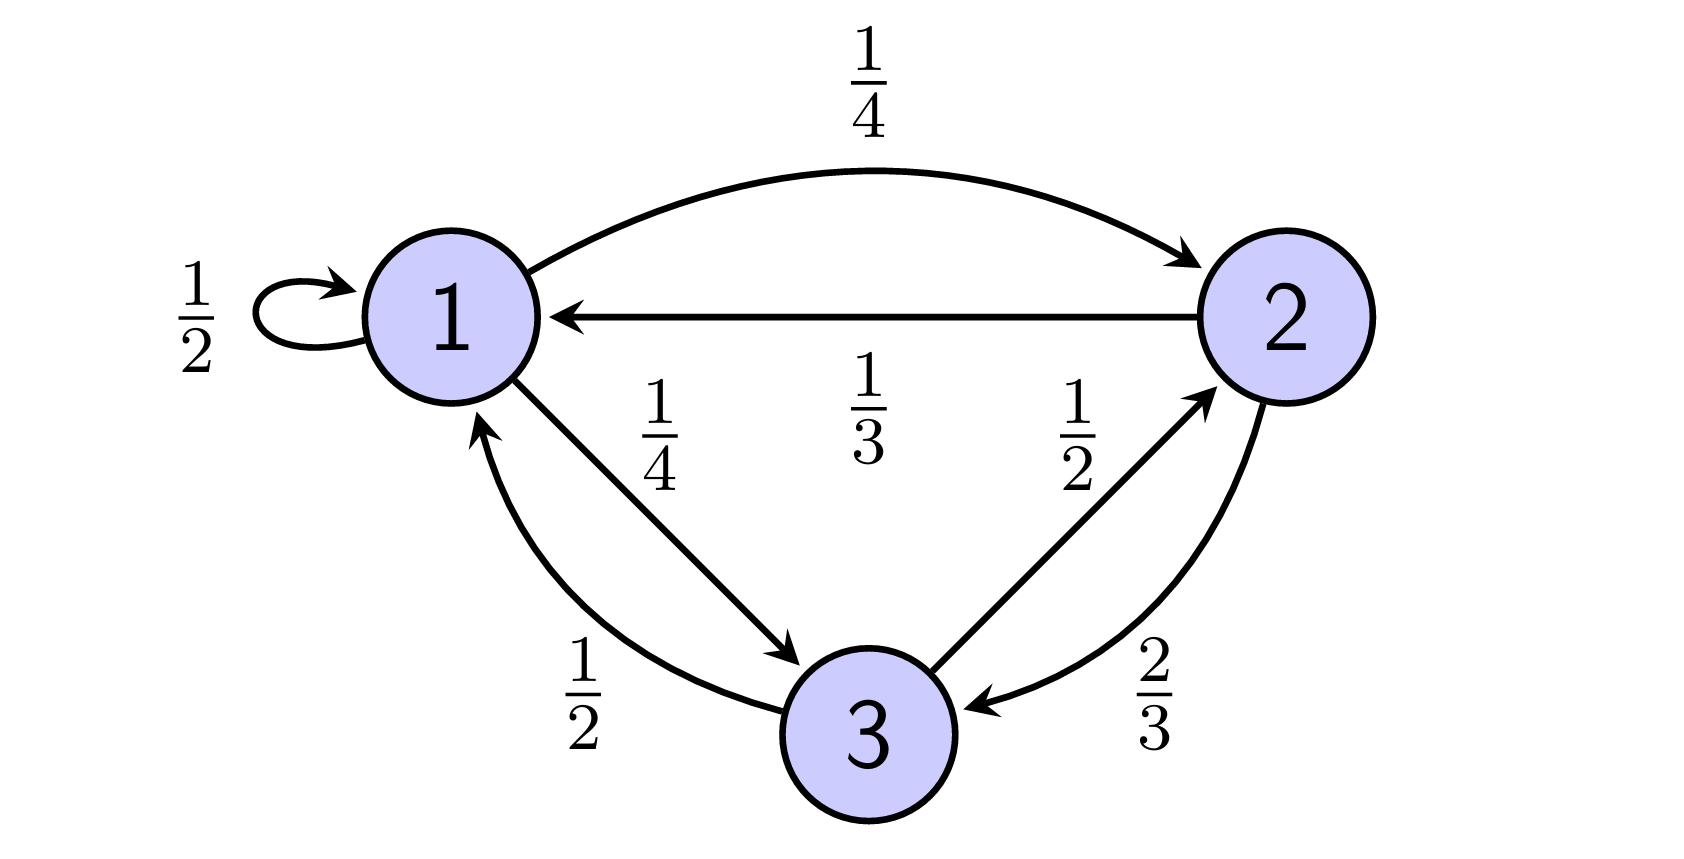
\includegraphics[width=0.5\linewidth]{figures/hw12 Markov chain.png}
\end{figure}
\begin{enumerate}[(a)]
    \item Find $P\left(X_3=3 \mid X_2=2\right)$ and $P\left(X_4=1 \mid X_3=2\right)$.
    \item If $P\left(X_0=2\right)=\frac{2}{5}$, find $P\left(X_0=2, X_1=3, X_2=1\right)$.
    \item Find $P\left(X_2=1 \mid X_0=2\right), P\left(X_2=2 \mid X_0=2\right)$, and $P\left(X_2=3 \mid X_0=2\right)$.
    \item Find $E\left(X_2 \mid X_0=2\right)$.
\end{enumerate}
\subsection{Solution}
For the Markov chain, we have the transition matrix
    $$
    P=\left[\begin{array}{ccc}
    \frac{1}{2} & \frac{1}{4} & \frac{1}{4} \\
    \frac{1}{3} & 0 & \frac{2}{3} \\
    \frac{1}{2} & \frac{1}{2} & 0
    \end{array}\right]
    $$
\begin{enumerate}[(a)]
    \item According to the transition matrix, we have
    $$
    P\left(X_3=3 \mid X_2=2\right)=\frac{2}{3}
    $$
    $$
    P\left(X_4=1 \mid X_3=2\right)=\frac{1}{3}
    $$
    \item We have
    $$
    P\left(X_0=2, X_1=3, X_2=1\right)=P\left(X_0=2\right) P\left(X_1=3 \mid X_0=2\right) P\left(X_2=1 \mid X_1=3\right)=\frac{2}{5} \times \frac{2}{3} \times \frac{1}{2}=\frac{2}{15}
    $$
    \item We are solving the probability of $X_2$ given $X_0$, so we can use the square of the transition matrix $P$ to get the transition matrix from $X_0$ to $X_2$:
    $$
    P^2=\left[\begin{array}{ccc}
    \frac{1}{2} & \frac{1}{4} & \frac{1}{4} \\
    \frac{1}{3} & 0 & \frac{2}{3} \\
    \frac{1}{2} & \frac{1}{2} & 0
    \end{array}\right]\left[\begin{array}{ccc}
    \frac{1}{2} & \frac{1}{4} & \frac{1}{4} \\
    \frac{1}{3} & 0 & \frac{2}{3} \\
    \frac{1}{2} & \frac{1}{2} & 0
    \end{array}\right]=\left[\begin{array}{ccc}
    \frac{11}{24} & \frac{1}{4} & \frac{7}{24} \\
    \frac{1}{2} & \frac{5}{12} & \frac{1}{12} \\
    \frac{5}{12} & \frac{1}{8} & \frac{11}{24}
    \end{array}\right]
    $$
    Thus, we have
    $
    P\left(X_2=1 \mid X_0=2\right)=\frac{1}{2}
    $
    $
    P\left(X_2=2 \mid X_0=2\right)=\frac{5}{12}
    $
    $
    P\left(X_2=3 \mid X_0=2\right)=\frac{1}{12}
    $
    \item We have
    $$
    E\left(X_2 \mid X_0=2\right)=1 \times P\left(X_2=1 \mid X_0=2\right)+2 \times P\left(X_2=2 \mid X_0=2\right)+3 \times P\left(X_2=3 \mid X_0=2\right)=\frac{1}{2}+\frac{5}{6}+\frac{1}{4}=\frac{19}{12}
    $$



\end{enumerate}

\end{homeworkProblem}

\newpage

\begin{homeworkProblem}[4]
Let the random variable $X \sim \mathcal{N}\left(\mu, \tau^2\right)$. Given $X=x$, random variables $Y_1, Y_2, \ldots, Y_n$ are i.i.d. and have the same conditional distribution, i.e., $Y_i \mid X=x \sim \mathcal{N}\left(x, \sigma^2\right)$. Define the sample mean $\bar{Y}$ as follows:

$$
\bar{Y}=\frac{Y_1+\cdots+Y_n}{n}
$$
\begin{enumerate}
    \item Find the posterior PDF of $X$ given $\bar{Y}$.
    \item Find the MAP (Maximum a Posterior Probability) estimates of $X$ given $\bar{Y}$.
    \item Find the MMSE estimates of $X$ given $\bar{Y}$. (We know that the MMSE of $X$ given $Y$ is given by $g(Y)=E[X \mid Y])$.
\end{enumerate}
\end{homeworkProblem}
\subsection{Solution}
\begin{enumerate}[(a)]
    \item

Using Bayes' theorem, the posterior PDF is:
\[
p(X \mid \bar{Y}) \propto p(\bar{Y} \mid X) p(X),
\]
where \( p(X) \) is the prior PDF of \( X \), i.e., \( X \sim \mathcal{N}(\mu, \tau^2) \),
\( p(\bar{Y} \mid X) \) is the likelihood, i.e., \( \bar{Y} \mid X = x \sim \mathcal{N}(x, \sigma^2 / n) \).\\
So we have
\[
p(\bar{Y} \mid X = x) = \frac{1}{\sqrt{2\pi \sigma^2 / n}} \exp\left( -\frac{n}{2\sigma^2} (\bar{Y} - x)^2 \right).
\]

\[
p(X = x) = \frac{1}{\sqrt{2\pi \tau^2}} \exp\left( -\frac{1}{2\tau^2} (x - \mu)^2 \right).
\]
Combining the likelihood and prior, we have the unnormalized posterior
\[
p(X \mid \bar{Y}) \propto \exp\left( -\frac{n}{2\sigma^2} (\bar{Y} - x)^2 - \frac{1}{2\tau^2} (x - \mu)^2 \right).
\]

Simplify the exponent, we have
\[
-\frac{n}{2\sigma^2} (\bar{Y} - x)^2 - \frac{1}{2\tau^2} (x - \mu)^2 = -\frac{1}{2} \left[ \left( \frac{n}{\sigma^2} + \frac{1}{\tau^2} \right)x^2 - 2 \left( \frac{n \bar{Y}}{\sigma^2} + \frac{\mu}{\tau^2} \right)x + \text{const} \right].
\]

This is quadratic in \( x \), so the posterior is 
\[
X \mid \bar{Y} \sim \mathcal{N}(\nu, \rho^2),
\]
where:
\[
\rho^2 = \frac{1}{\frac{n}{\sigma^2} + \frac{1}{\tau^2}}, \quad \nu = \rho^2 \left( \frac{n \bar{Y}}{\sigma^2} + \frac{\mu}{\tau^2} \right).
\]

\item The MAP estimate of \( X \) given \( \bar{Y} \) is the mode of the posterior, which is the mean of the posterior. So the MAP estimate is:
\[
\hat{X}_{\text{MAP}} = \nu = \rho^2 \left( \frac{n \bar{Y}}{\sigma^2} + \frac{\mu}{\tau^2} \right) = \frac{\frac{n}{\sigma^2} \bar{Y} + \frac{1}{\tau^2} \mu}{\frac{n}{\sigma^2} + \frac{1}{\tau^2}}.
\]

\item The MMSE estimate is given by the conditional expectation
\[
\hat{X}_{\text{MMSE}} = E[X \mid \bar{Y}] = \nu = \rho^2 \left( \frac{n \bar{Y}}{\sigma^2} + \frac{\mu}{\tau^2} \right) = \frac{\frac{n}{\sigma^2} \bar{Y} + \frac{1}{\tau^2} \mu}{\frac{n}{\sigma^2} + \frac{1}{\tau^2}}.
\]




\end{enumerate}


\end{document}

%4. Let $\boldsymbol{X}=\left(X_{1}, \ldots, X_{n}\right)$ be a random sample from the distribution $\mathcal{N}\left(\mu, \sigma^{2}\right)$, where both $\mu$ and $\sigma^{2}$ are unknown constants. Suppose the observed data is $\boldsymbol{x}=\left(x_{1}, \ldots, x_{n}\right)$, find both $\hat{\mu}$ (estimate of $\mu$ ) and $\hat{\sigma}^{2}$ (estimate of $\sigma^{2}$ ) through the MLE (Maximum Likelihood Estimation) rule.\\
5. Given a coin with the probability $p$ of landing heads. $p$ is unknown and we need to estimate its value through data. In our data collection model, we have $n$ independent tosses, result of each toss is either Head or Tail. Let $X$ denote the number of heads in the total $n$ tosses. Now we conduct experiments to collect data and find $X=k$. Then we need to find $\hat{p}$, the estimation of $p$.\\
(a) Assume $p$ is an unknown constant. Find $\hat{p}$ through the MLE (Maximum Likelihood Estimation) rule.\\
(b) Assume $p$ is a random variable with a prior distribution $p \sim \operatorname{Beta}(a, b)$, where $a$ and $b$ are known constants. Find $\hat{p}$ through the MAP (Maximum a Posterior Probability) rule.\\
(c) Assume $p$ is a random variable with a prior distribution $p \sim \operatorname{Beta}(a, b)$, where $a$ and $b$ are known constants. Find $\hat{p}$ through the posterior mean rule.\\
6. Two chess players, Vishy and Magnus, play a series of games. Given $p$, the game results are i.i.d. with probability $p$ of Vishy winning, and probability $q=1-p$ of Magnus winning (assume that each game ends in a win for one of the two players). But $p$ is unknown, so we will treat it as an r.v. To reflect our uncertainty about $p$, we use the prior $p \sim \operatorname{Beta}(a, b)$, where a and b are known positive integers and $a \geq 2$.\\
(a) Find the expected number of games needed in order for Vishy to win a game (including the win). Simplify fully; your final answer should not use factorials or $\Gamma$.\\
(b) Explain in terms of independence vs. conditional independence the direction of the inequality between the answer to (a) and $1+E(G)$ for $G \sim \operatorname{Geom}\left(\frac{a}{a+b}\right)$.\\
(c) Find the conditional distribution of $p$ given that Vishy wins exactly 7 out of the first 10 games.
